\section{Implementation options}
We present below different possible implementations of the previous diagram.

\subsection{Sensors}
The tables below show the different options for the four sensors required in our HPCS system.

\begin{figure}[h]
    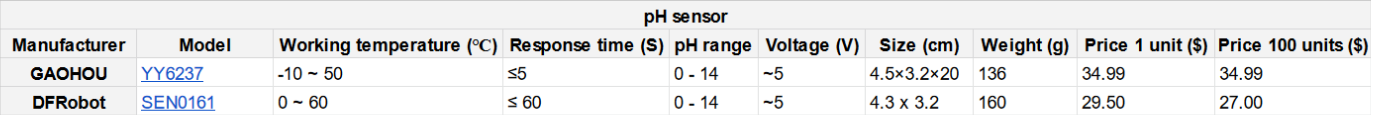
\includegraphics[width=\linewidth]{images/ph-sensor-comparison.png}
    \caption{pH Sensor comparison}
    \label{fig:pH Sensor Comparison}
\end{figure}

\begin{figure}[h]
    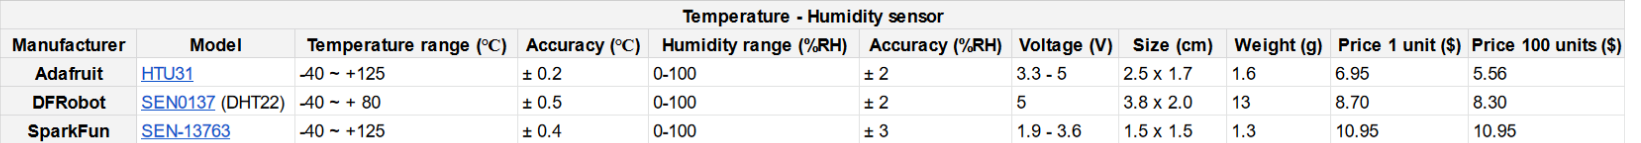
\includegraphics[width=\linewidth]{images/temp-hum-sensor-comparison.png}
    \caption{Temperature - Humidity Sensor comparison}
    \label{fig:Temperature - Humidity Sensor Comparison}
\end{figure}

\begin{figure}[h]
    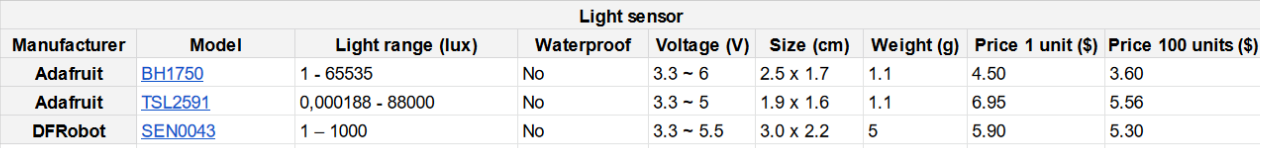
\includegraphics[width=\linewidth]{images/light-sensor-comparison.png}
    \caption{Light Sensor comparison}
    \label{fig:Light Sensor Comparison}
\end{figure}
\subsection{MCU board}
\subsection{Battery}
The table below compares some non-rechargeable button cell batteries that would be suitable for our system \cite{b7}.
They are very similar to each other but can differ in their lifetime and size. Prices are those of the seller Ace Hardware.
\begin{figure}[h]
    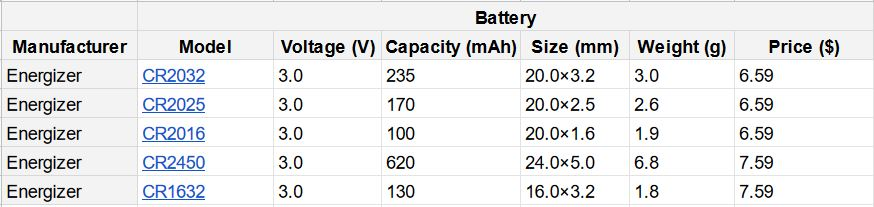
\includegraphics[width=\linewidth]{images/battery-comparison.jpg}
    \caption{Battery comparison}
    \label{fig:Battery Comparison}
\end{figure}

\subsection{Computing platforms}
\subsubsection{Arduinos and alternative platforms}
\subsubsection{Edge platforms}
\subsubsection{Cloud options}
The available hosting options options, cloud-wise, are all quite similar. They all
provide a platform to host any web component of the application and database services
to store the data. The main differences are in pricing and complexity of usage and
maintenance. The table below shows the main differences between the two main
options considered: AWS and Azure. The table is based on the assumption
that the web component will be hosted on a Linux server and the database will be
hosted in a non-relational database (NoSQL) service (e.g. MongoDB, DynamoDB, etc.),
ignoring free tier options (they are not relevant for our purposes, as the system will
eventually be deployed in a real-world scenario where the limitations of the free
tier are not relevant) and with yearly contracts in mind.

\begin{table}
    \centering
    \begin{tabularx}{\columnwidth}{|l|c|c|c|}
        \hline
        \textbf{Feature} & \textbf{AWS} & \textbf{Azure} \\
        \hline
        Database Pricing &
            \$0.25 per GB per month + \$1.25 per million writes + \$0.25 per million reads & 
            \$0.25 per GB per month + \$0.28 per million requests \\
        \hline
        Linux Server Pricing &
            \$10 per month (T2.small instance)& 
            \$10 per month (B1ms instance) \\
        \end{tabularx}
\end{table}

As seen, the main difference is in the database pricing. AWS is cheaper for reads,
but Azure is cheaper for writes. The Linux server pricing is the same for both options
at the size we're looking at. Additionally, Azure offers an IoT Hub service that
could replace some of the functionality of the web component.
\subsection{Data format}

\subsection{Device-Edge communication protocols}
The high latency brought on by a sensor device's mobility for remote monitoring in edge-based IoT applications can have detrimental effects including erroneous analysis and poor service quality \cite{b5}. In order to reduce latency and while maintaining a connection, high quality of service, and energy efficiency, mobility support approaches are necessary. Therefore for our IOT solution we will be using a wireless connection for the communication Device-edge: Bluetooth. 
\subsubsection{Bluetooth types}
Bluetooth is a short-range wireless technology medium used for exchanging data between two electronic devices over a short distance. 
UHF radio waves, often known as short wave radio, are used by Bluetooth exchange to create a Personal Area Network employing radio bands ranging from 2.402 GHz to 2.480 GHz.

Since there are two Bluetooth types, Bluetooth Classic and Bluetooth Low Energy (BLE), all Bluetooth devices can be divided into these two categories. On the one hand, wireless speakers, headsets, and automotive infotainment systems frequently use the Bluetooth Classic standard. Bluetooth Low Energy, on the other hand, is more common in applications that focus on battery consumption and transfer small amounts of data less frequently. To put it another way, BLE is frequently found in battery-operated gadgets like cell phones, sensor devices, etc. While keeping a similar communication range to Bluetooth Classic, Bluetooth Low Energy survives on lower power consumption and costs. This is in contrast to Bluetooth Classic, which uses a lot of energy.

\begin{table}[htbp]
    \centering
    \begin{tabular}{|c|c|c|}
        \hline
        \textbf{Bluetooth} & \textbf{Classic} & \textbf{Low Energy}  \\
        \hline
        Data payload throughput & 2Mbps & ~100 kbps\\
        \hline
        Robustness & Strong & Strong\\
        \hline
        Range & Up to 1000m & Up to 250m\\
        \hline
        Local System density & Strong & Strong\\
        \hline
        Large scale network & Weak & Good\\
        \hline
        Low latency & Strong & Strong\\
        \hline
        Connection set-up speed & Weak & Strong\\
        \hline
        Power consumption & Good & Very strong\\
        \hline
        Cost & Good & Strong \\
        \hline
        \end{tabular}
    \caption{Comparison between Bluetooth Classic and Low Energy (BLE) \cite{b4}}
    \label{tab:my_label}
\end{table}

\subsubsection{Bluetooth in IOT}
By keeping IoT devices in sleep mode while not in use and allowing users to wake them up when connected or reconnected, Bluetooth Low Energy in IoT can help IoT devices save energy. Because IoT BLE apps can swiftly pair and reconnect with devices in six milliseconds as opposed to traditional Bluetooth applications that must wait six seconds or longer, Bluetooth Low Energy is perfect for IoT applications.

Considering the usage of both Bluetooth options as well as their specificities summarized in the comparison table, why we have decided to use Bluetooth Low Energy for our project through the BLEPeripheral library.

\subsection{Edge-Cloud communication protocols}
IoT Hub allows devices to use alternative protocols for Edge-Cloud communications, such as HTTP/HTTPS, MQTT and AMQP \cite{b1}. In this section we will try to compare each of those protocols and see which ones would suit our project the best.

\subsubsection{MQTT} is a communication protocol with features specifically targeted at IoT solutions. With a small code footprint and low network bandwidth requirements, it is designed as a lightweight publish/subscribe messaging transport that is perfect for linking remote devices.\\
The ease and flexibility with which solutions can be developed is one of MQTT's best features. Multiple clients can produce and share information with back end systems and each other thanks to the publish-subscribe paradigm.

\subsubsection{AMQP} is a messaging protocol which was created to be a non-proprietary method of connecting applications and was not targeted at IoT solutions. It is used on field and cloud gateways to take advantage of connection multiplexing across devices. One of its benefits is that, while being a complicated messaging system, it is lightweight, has little overhead, and uses minimal CPU and RAM. \\
For general purpose message queuing, AMQP offers more flexibility than MQTT, at the expense of some efficiency and complexity.However it places a strong emphasis on message delivery that adds to the overhead eventually.

\subsubsection{HTTPS} is a heavy text-based protocol working on a request/response model. A client sends a request to the server, and the server sends back a response.\\
The main benefit of HTTPS for use in IoT is its familiarity to developers which are likely to have had implemented web solutions of one kind or another. A consequence of this is the availability of client libraries and servers. Additionally it is scalable and can be used with multiple devices.\\


As MQTT was designed for IoT solutions it fits many more IoT scenarios than its counterparts. \\
Will and retained messages are two MQTT capabilities that AMQP does not directly support \cite{b2}. Moreover, mistakes might be made when configuring routing topologies of AMQP, which is impossible in the more straightforward MQTT environment.\\
The cost of connection setup is a small drawback of MQTT versus HTTPS. This overhead may be higher than HTTPS if each TCP session only sends one message. However, because this is not a typical IoT case, MQTT soon becomes advantageous when several messages are transmitted and received within the same TCP session \cite{b3}. HTTPS also needs more power and memory to function than MQTT.\\

Considering the advantages and disadvantages of the different protocols listed above and taking into account the comparison table.
It seems like the best protocols to implement for the HPCS would be MQTT or HTTPS protocols with a preference for MQTT.

\newpage
\begin{table*}
    \caption{Communication protocols comparison}
    \begin{center}
    \renewcommand{\arraystretch}{2}
    \begin{tabular}{|p{3cm}|p{4.5cm}|p{4.5cm}|p{4.5cm}|}
    \hline
    \textbf{{Protocols}}& \textbf{\textit{AMQP}}& \textbf{\textit{MQTT}}& \textbf{\textit{HTTP}} \\
    \hline
    Full Name & Advanced Message Queuing Protocol & MQTT (the OASIS standardization group decided it would not stand for anything) & Hyper Text Transfer Protocol\\
    \hline
    Architecture & Queues, multicast (fanout), publish subscribe, request reply & Publish subscribe (MQTT does have a request/reply mode as well) & Request response\\
    \hline
    Command Targets & Exchanges, Queues & Topics & URIs\\
    \hline
    Underlying Protocol & TCP/IP & TCP/IP & TCP/IP\\
    \hline
    Secure connections & TLS + username/password (SASL support possible) & TLS + username/password (SASL support possible) & TLS + username/password (SASL support possible)\\
    \hline
    Client observability & Unknown connection status & Known connection status (will messages) & Unknown connection status\\
    \hline
    Messaging mode & Synchronous and asynchronous & Asynchronous, event-based & Synchronous\\
    \hline
    Messaging queuing & Core capability, flexible configuration & The broker can queue messages for disconnected subscribers & Application needs to implement\\
    \hline
    Message overhead & 8 bytes (general frame format) & 2 bytes minimum (header data can be binary) & 8 bytes minimum (header data is text - compression possible)\\
    \hline
    Message Size & 2GB theoretical, 128MB max recommended & 256MB maximum & No limit but 256MB is beyond normal use cases anyway.\\
    \hline
    Content type & Any (binary) & Any (binary) & Text (Base64 encoding for binary)\\
    \hline
    Topic matching & Level separator: . Wildcards: \* \# & Level separator: / Wildcards: + \# & - \\
    \hline
    Reliability & Two qualities of service: -without acks (=0) - with acks (=1) & Three qualities of service: 0 - fire and forget 1 - at least once 2 - once and only once & Has to be implemented in the application\\
    \hline
    Connection "multiplexing" & Yes - channels & No & -\\
    \hline
    Message attributes & Yes & MQTT 5.0 only & -\\
    \hline
    Object persistence & Yes & Yes & -\\
    \hline
    \end{tabular}
    \label{tab-1}
    \end{center}
    \end{table*}